\documentclass[xcolor=dvipsnames,handout]{beamer}

\usetheme{Madrid}
\setbeamertemplate{navigation symbols}{}

\usepackage{mpctools}

% Need to make code a bit smaller.
\lstdefinestyle{beameroctave}{
    style=octave,
    basicstyle=\ttfamily\scriptsize,
    deletekeywords={filter},
}
\lstset{style=beameroctave}

\newcommand{\seq}{\mathbf}
\newcommand{\useq}{\seq{u}}
\newcommand{\xseq}{\seq{x}}
\newcommand{\bbX}{\mathbb{X}}
\newcommand{\bbZ}{\mathbb{Z}}

\usepackage{tikz}
\usetikzlibrary{arrows.meta,decorations.pathmorphing,calc}

\title[MPCTools]{\Huge \mpctools{} \\ \LARGE Nonlinear MPC using \casadi{}}
\author[Michael Risbeck]{\LARGE Michael Risbeck}
\date[April 5th, 2017]{\Large April 5th, 2017}

\begin{document}

\frame{\titlepage}

\begin{frame}[fragile]{Nonlinear MPC}
    \renewcommand{\emph}[1]{\text{\textcolor{Blue}{#1}}}
    By now, you're (hopefully) familiar with the standard nonlinear MPC setup
    %
    \begin{align*}
        \min_{\xseq, \useq} \quad & \sum_{k = 0}^{N - 1} \ell(x(k),u(k)) & \emph{Stage Costs} \\[-1em]
        & \qquad\qquad + V_f(x(N)) & \emph{Terminal Cost} \\
        \text{s.t.} \quad & x(k + 1) = f(x(k), u(k))\ & \emph{Model}\\
        & (x(k), u(k)) \in \bbZ & \emph{State/input Constraints} \\
        & x(N) \in \bbX_f & \emph{Terminal Set} \\
        & x(0) = x & \emph{Initial Condition}
    \end{align*} \pause
    
    \vspace{-1em}
    
    To solve example problems, we want fast algorithmic differentiation attached to powerful NLP solvers.
    %
    \begin{itemize}
        \item \casadi{} provides both of these via Octave (and Matlab)
        \item Let's see an example
    \end{itemize}
\end{frame}

\begin{frame}[fragile]{\casadi{} Basics}
    Consider the simple example of a hanging spring.
    \begin{columns}
        \begin{column}{.4\textwidth}
            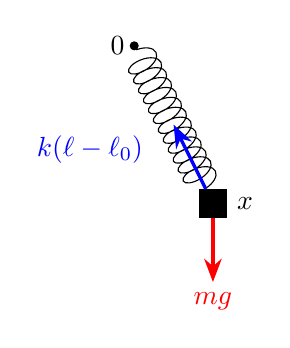
\begin{tikzpicture}
                [
                    dot/.style={circle,fill=black,draw=black,inner sep=0,minimum size=0.1cm},
                    box/.style={rectangle,fill=black,draw=black,inner sep=0,minimum size=0.35cm},
                    spring/.style={draw=black,decorate,decoration={coil,amplitude=6pt,segment length=4pt}},
                    vector/.style={-{Stealth[fill=#1]},very thick,draw=#1,text=#1},
                ]
                \draw (0,0) node[dot] (o) {}
                      node[left] {$0$};
                \draw (1,-2) node[box] (b) {}
                      (b.east) node[right] {$x$};
                \draw[spring] (o) -- (b);
                \draw[vector=red] (b) -- ++(0,-1cm) node[below] {$mg$};
                \draw[vector=blue] (b) -- ($0.5*(b) + 0.5*(o)$)
                    node[below left,xshift=-0.25cm] {$k(\ell - \ell_0)$};
            \end{tikzpicture} \pause
            
            \color{black} % Without this, the black text below doesn't show up.
            Total energy is minimized at equilibrium:
            %
            \begin{align*}
                E & = \textcolor{blue}{k(\ell - \ell_0)^2}
                      + \textcolor{red}{mgh} \\
                & = \textcolor{blue}{k}(\|x\| - \textcolor{blue}{\ell_0})^2
                    + \textcolor{red}{mg}x_2
            \end{align*}
        \end{column} \pause
        \begin{column}{.55\textwidth}
            \begin{lstlisting}[gobble=16]
                % Example use of CasADi
                k = 10; L0 = 1; g = 9.8; m = 1;
                
                x = casadi.SX.sym('x', 2);
                
                E = k*(norm(x) - L0)^2 ...
                    + m*g*x(2);
                
                nlp = struct('x', x, 'f', E);
                solver = ...
                    casadi.nlpsol('springsolver', ...
                                  'ipopt', nlp);
                
                solution = solver('x0', [2; -1]);
                
                % Equilibrium position:
                disp(solution.x);
                % >> DM([6.49685e-12, -1.49])
            \end{lstlisting}
        \end{column}
    \end{columns}
\end{frame}

\begin{frame}{What's in \casadi?}
    \textcolor{red}{Cas}\textcolor{blue}{ADi} = \textcolor{red}{C}omputer \textcolor{red}{a}lgebra \textcolor{red}{s}ystem + \textcolor{blue}{A}lgorithmic \textcolor{blue}{Di}fferentiation
    \begin{itemize}
        \item<+-> Symbolic algebraic expression core
        \begin{itemize}
            \item Can construct algebraic expressions and perform some simplification
            \item Not a general-purpose computer algebra system
        \end{itemize}
        \item<+-> State-of-the-art ODE and DAE integrators (e.g., CVODES, IDAS)
        \begin{itemize}
            \item Can take derivatives of these objects!
        \end{itemize}
        \item<+-> Links to state-of-the-art solvers (e.g., IPOPT, qpOASES)
        \begin{itemize}
            \item Provides exact first and second derivatives
            \item Initial support for discrete variables
        \end{itemize}
        \item<+-> C code generation
    \end{itemize} \pause
    
    See \smallurl{casadi.org} for more information. \pause
    
    \bigskip
    
    To paraphrase Spiderman: \pause
    \begin{quote}
        With great power comes great possibility for people to write unreadable and unmaintainable code!
    \end{quote}
\end{frame}

\begin{frame}[fragile]{From official CasADi Examples}
    \begin{columns}
        \begin{column}{.65\textwidth}
            \begin{lstlisting}[basicstyle=\ttfamily\fontsize{6}{8}\selectfont,gobble=16]
                for j=1:d+1
                  % Construct Lagrange polynomials to get the
                  % polynomial basis at the collocation point
                  coeff = 1;
                  for r=1:d+1
                    if r ~= j
                      coeff = conv(coeff, [1, -tau_root(r)]);
                      coeff = coeff / (tau_root(j)-tau_root(r));
                    end
                  end
                  % Evaluate the polynomial at the final time to get
                  % the coefficients of the continuity equation
                  D(j) = polyval(coeff, 1.0);
                
                  % Evaluate the time derivative of the polynomial
                  % at all collocation points to get the coefficients
                  % of the continuity equation
                  pder = polyder(coeff);
                  for r=1:d+1
                    C(j,r) = polyval(pder, tau_root(r));
                  end
                
                  % Evaluate the integral of the polynomial to get the
                  % coefficients of the quadrature function
                  pint = polyint(coeff);
                  B(j) = polyval(pint, 1.0);
                end
            \end{lstlisting}
        \end{column}
        \begin{column}{.3\textwidth}
            Things can escalate pretty quickly. \pause
            
            \bigskip
            
            We don't want everyone writing this themselves!
        \end{column}
    \end{columns}
\end{frame}

\begin{frame}{What do we want?}
    \begin{itemize}
        \item We want to solve nonlinear MPC problems.
        \item \casadi{} is more robust than our in-house software
        \item However, setting up an MPC problem in CasADi takes a lot of code
        \item Everyone copy/pasting their own code is bad
        \item A simpler interface means we can save a lot of time
    \end{itemize}
\end{frame}

\begin{frame}{Enter \mpctools}
    An Octave package (usually Matlab-compatible)
    \begin{itemize}
        \item Download from \bitbucketlink
        \item Put the \texttt{mpctools} folder somewhere and add it to Octave's path
        \item Running \lstinline!mpc = import_mpctools()! gives access to functions via \lstinline!mpc.*!
        \begin{itemize}
            \item Can also call functions via \lstinline!mpctools.*! without import
        \end{itemize}
    \end{itemize} \pause
    
    \medskip
    
    Comes with cheatsheet and full documentation (in the \texttt{doc} folder).
    \begin{itemize}
        \item Should get you started writing your own code.
    \end{itemize} \pause
    
    \medskip
    
    Also includes a bunch of example files, e.g.,
    \begin{itemize}
        \item \texttt{cstr.m}: Example 1.11 using \casadi{} integrators and linearization
        \item \texttt{vdposcillator.m}: Example of linear vs. nonlinear MPC.
        \item \texttt{cstr\_startup.m}: Nonlinear startup for Example 1.11 system.
    \end{itemize}
\end{frame}

\begin{frame}[fragile]{System Model}
    Start by defining the system model as an Octave function.
    
    \begin{lstlisting}[gobble=8]
        function rhs = cstrode(x, u, p, pars)
            % Nonlinear ODE model for reactor.
            c = x(1); T = x(2); h = x(3) + eps();
            
            Tc = u(1); F = u(2);
            
            F0 = p(1);
            
            k = pars.k0*exp(-pars.E/T);
            rate = k*c;
            
            dcdt = F0*(pars.c0 - c)/(pars.A*h) - rate;
            dTdt = F0*(pars.T0 - T)/(pars.A*h) ...
                   - pars.DeltaH/pars.rhoCp*rate ...
                   + 2*pars.U/(pars.r*pars.rhoCp)*(Tc - T); 
            dhdt = (F0 - F)/pars.A;
            
            rhs = [dcdt; dTdt; dhdt];
        end%function
    \end{lstlisting}
\end{frame}

\begin{frame}[fragile]{System Simulation}
    The nonlinear system can be simulated using CasADi \texttt{integrator} objects, created via a convenient wrapper.
        
    \begin{lstlisting}[gobble=8]
        % Turn into casadi function and simulator.
        ode = @(x, u, p) cstrode(x, u, p, pars);
        ode_casadi = mpc.getCasadiFunc(ode, [Nx, Nu, Np], ...
                                       {'x', 'u', 'p'}, {'ode'});
        cstrsim = mpc.getCasadiIntegrator(ode, Delta, [Nx, Nu, Np], ...
                                          {'x', 'u', 'p'}, {'cstr'});
        
        % Simulate with nonlinear model.
        x(:,t+1) = full(cstr(x(:,t), u(:,t), d(:,t)));
    \end{lstlisting} \pause
    
    \bigskip
    
    Note that \lstinline!cstr! returns \casadi{} \lstinline!DM! objects
    \begin{itemize}
        \item ``Double Matrix'', \casadi's internal (numeric) Matrix type
        \item Call to \lstinline!full()! converts to native Octave matrix
    \end{itemize}
\end{frame}

\begin{frame}[fragile]{Linear Unconstrained Control}
    \begin{columns}[t]
        \begin{column}{.475\textwidth}
            Set up linear controller and estimator.
            
            \begin{lstlisting}[gobble=16,basicstyle=\ttfamily\fontsize{6}{8}\selectfont]
                % Get linearized model.
                model = mpc.getLinearizedModel( ...
                            ode_casadi, {xs, us, ps}, ...
                            {'A', 'B', 'Bp'}, Delta);
                A = model.A;
                B = model.B;
                
                % Find LQR.
                [K, Pi] = dlqr(A, B, Q, R);
                K = -K; % Note sign convention.
                
                % Find Kalman Filter.
                kf = mpc.KalmanFilter('A', A, ...
                        'B', B, 'C', C, 'Bd', Bd, ...
                        'Cd', Cd, 'Qw', Qw, ...
                        'Rv', Rv, 'contvars', [1, 3]);
            \end{lstlisting}
        \end{column} \pause
        \begin{column}{.475\textwidth}
            Simulate closed-loop.
            
            \begin{lstlisting}[gobble=16,basicstyle=\ttfamily\fontsize{6}{8}\selectfont]
                for i = 1:(Nsim + 1)
                    % Take measurement.
                    y(:,i) = C*x(:,i) + v(:,i);
                    
                    % Advance state measurement.
                    [xhat(:,i), dhat(:,i)] = ...
                        kf.filter(y(:,i), xhatm(:,i), ...
                                  dhatm(:,i));
                    
                    % Use steady-state target selector.
                    [xtarg(:,i), utarg(:,i)] = ...
                        kf.target(ysp(:,i));
                    
                    % Apply control law.
                    u(:,i) = K*(xhat(:,i) - xtarg(:,i)) ...
                             + utarg(:,i);
                    
                    % Evolve plant.
                    x(:,i + 1) = full(cstrsim(x(:,i), ...
                                   u(:,i), p(:,i)));
                    
                    % Advance state estimates
                    [xhatm(:,i + 1), dhatm(:,i + 1)] = ...
                        kf.predict(u(:,i), xhat(:,i), ...
                                   dhat(:,i));
                end
            \end{lstlisting}
        \end{column}
    \end{columns}
\end{frame}

\begin{frame}{Results}
    \begin{center}
        \includegraphics[width=\textwidth]{cstr.pdf}
    \end{center}
\end{frame}


\begin{frame}{What can we do with \mpctools?}
    \begin{itemize}
        \item Discrete-time linear MPC
        \item Discrete-time nonlinear MPC
        \begin{itemize}
            \item Explicit models
            \item Runge-Kutta discretization
            \item Collocation
            \item DAE systems
        \end{itemize}
        \item Discrete-time nonlinear MHE
        \begin{itemize}
            \item Explicit models
            \item Runge-Kutta discretization
            \item Collocation
        \end{itemize}
        \item Steady-state target calculation
        \item Basic plotting
    \end{itemize}
\end{frame}

\begin{frame}[fragile]{Example: Van der Pol Oscillator}
    \begin{tikzpicture}[overlay, remember picture]
        \useasboundingbox (current page.north west) -- (current page.south east);
        \draw (9.25,-4.75) node[draw=black,fill=white,rounded corners, align=center]
            {System Model: \\[0.5em]
             $\displaystyle
              \frac{dx}{dt} =
                  \begin{pmatrix}
                      (1 - x_2)^2x_1 - x_2 + u \\
                       x_1
                   \end{pmatrix}
            $};
    \end{tikzpicture}
    
    \vspace{-2em}
    
    \begin{lstlisting}[gobble=8,basicstyle=\ttfamily\fontsize{6}{8}\selectfont]
        % Define nonlinear and linearized models.
        ode = @(x, u) [(1 - x(2).^2)*x(1) - x(2) + u(1); x(1)];
        vdp = mpctools.getCasadiIntegrator(ode, Delta, [Nx, Nu], {'x', 'u'}, {'vdp'});
        fnonlin = mpctools.getCasadiFunc(ode, [Nx, Nu], {'x', 'u'}, {'vdprk4'}, ...
                                         'rk4', true(), 'Delta', Delta);
        linmodel = mpctools.getLinearizedModel(ode, {zeros(Nx, 1), zeros(Nu, 1)}, ...
                                               {'A', 'B'}, Delta);
        Flin = mpctools.getCasadiFunc(@(x, u) linmodel.A*x + linmodel.B*u, [Nx, Nu], ...
                                      {'x', 'u'}, {'vdplin'});
        
        % Define objective functions.
        stagecost = @(x, u) x'*x + u'*u;
        l = mpctools.getCasadiFunc(stagecost, [Nx, Nu], {'x', 'u'}, {'l'});
        
        termcost = @(x) 10*x'*x;
        Vf = mpctools.getCasadiFunc(termcost, [Nx], ...
                                    {'x'}, {'Vf'});
        
        % Set bounds.
        lb = struct('u', -0.75*ones(Nu, Nt));
        ub = struct('u', ones(Nu, Nt));
        
        % Build solvers.
        N = struct('x', Nx, 'u', Nu, 't', Nt);
        kwargs = struct('l', l, 'Vf', Vf, 'N', N, 'lb', lb, 'ub', ub);
        solvers = struct();
        solvers.LMPC = mpctools.nmpc('f', Flin,'**', kwargs);
        solvers.NMPC = mpctools.nmpc('f', fnonlin, '**', kwargs);
    \end{lstlisting}
\end{frame}

\begin{frame}{Simulation Results}
    For this problem, nonlinear MPC performs slightly better.
    \begin{itemize}
        \item The computation isn't much more time-consuming because of the power of \casadi.
        \item The problem isn't difficult to set up because of \mpctools.
    \end{itemize}
    \begin{center}
        \includegraphics[width=\textwidth]{vdposcillator.pdf}
    \end{center}
\end{frame}

\begin{frame}{More Complicated Example}

Using \mpctools{}, we can replace the LQR and KF from Example 1.11 with nonlinear MPC and MHE.

\begin{itemize}
    \item \texttt{cstr\_startup.m} shows basic structure and a setpoint change.
    \item \texttt{cstr\_nmpc\_nmhe.m} shows steady-state target finding and NMHE.
    \item See the cheatsheet for important functions and syntax.
\end{itemize}

\end{frame}

\begin{frame}{\texttt{cstr\_startup.m}}
    Here, nonlinear MPC knows to be less aggressive.
    \begin{center}
        \includegraphics[width=\textwidth]{cstr_startup.pdf}
     \end{center}
\end{frame}


\begin{frame}{What can't we do?}
    \begin{itemize}
        \item True continuous-time formulation
        \begin{itemize}
            \item Continuous-time models with explicit time dependence are not supported
            \item Quadrature for continuous-time objective function is available via collocation or RK4
        \end{itemize} \pause
        \item Quality guess generation
        \begin{itemize}
            \item Solve sequence of smaller problems
            \item Use as initial guess for large problem
            \item Must do by hand
        \end{itemize} \pause
        \item Stochastic MPC \pause
        \item Robust MPC
    \end{itemize}
\end{frame}

\begin{frame}{That's all, folks!}
    \begin{itemize}
        \item For questions, comments, etc., email \smallurl{risbeck@wisc.edu}
        \item For bugs or feature requests, open an issue on Bitbucket
        \begin{itemize}
            \item \bitbucketlink
        \end{itemize}
    \end{itemize}
    
    \bigskip
    
    \begin{columns}
        \begin{column}{0.475\textwidth}
            \includegraphics[width=\textwidth]{ballmaze.pdf}
        \end{column}
        \begin{column}{0.475\textwidth}
            \includegraphics[width=\textwidth]{econmpc.pdf}
        \end{column}
    \end{columns}
\end{frame}

\end{document}
